\section{Research Methods}

\subsection{Part One}

Lorem ipsum dolor sit amet, consectetur adipiscing elit. Morbi
malesuada, quam in pulvinar varius, metus nunc fermentum urna, id
sollicitudin purus odio sit amet enim. Aliquam ullamcorper eu ipsum
vel mollis. Curabitur quis dictum nisl. Phasellus vel semper risus, et
lacinia dolor. Integer ultricies commodo sem nec semper.

\subsection{Part Two}

Etiam commodo feugiat nisl pulvinar pellentesque. Etiam auctor sodales
ligula, non varius nibh pulvinar semper. Suspendisse nec lectus non
ipsum convallis congue hendrerit vitae sapien. Donec at laoreet
eros. Vivamus non purus placerat, scelerisque diam eu, cursus
ante. Etiam aliquam tortor auctor efficitur mattis.

\section{Online Resources}

Nam id fermentum dui. Suspendisse sagittis tortor a nulla mollis, in
pulvinar ex pretium. Sed interdum orci quis metus euismod, et sagittis
enim maximus. Vestibulum gravida massa ut felis suscipit
congue. Quisque mattis elit a risus ultrices commodo venenatis eget
dui. Etiam sagittis eleifend elementum.

Nam interdum magna at lectus dignissim, ac dignissim lorem
rhoncus. Maecenas eu arcu ac neque placerat aliquam. Nunc pulvinar
massa et mattis lacinia.

\section{End of the appendix}
Always include figures and table of full width of both column like below with \begin{verbatim}
    \begin{figure*}
        \centering
        \includegraphics{}
        \caption{Caption}
        \label{fig:my_label}
    \end{figure}
\end{verbatim}, otherwise images will not be rendered.

\begin{figure*}[!hb]
    \centering
    %\includegraphics[trim={0.2cm 0 5.3cm 3.6cm},clip,scale=0.32]{images/category-wise-distr/curl_vendor_categorization.pdf}
    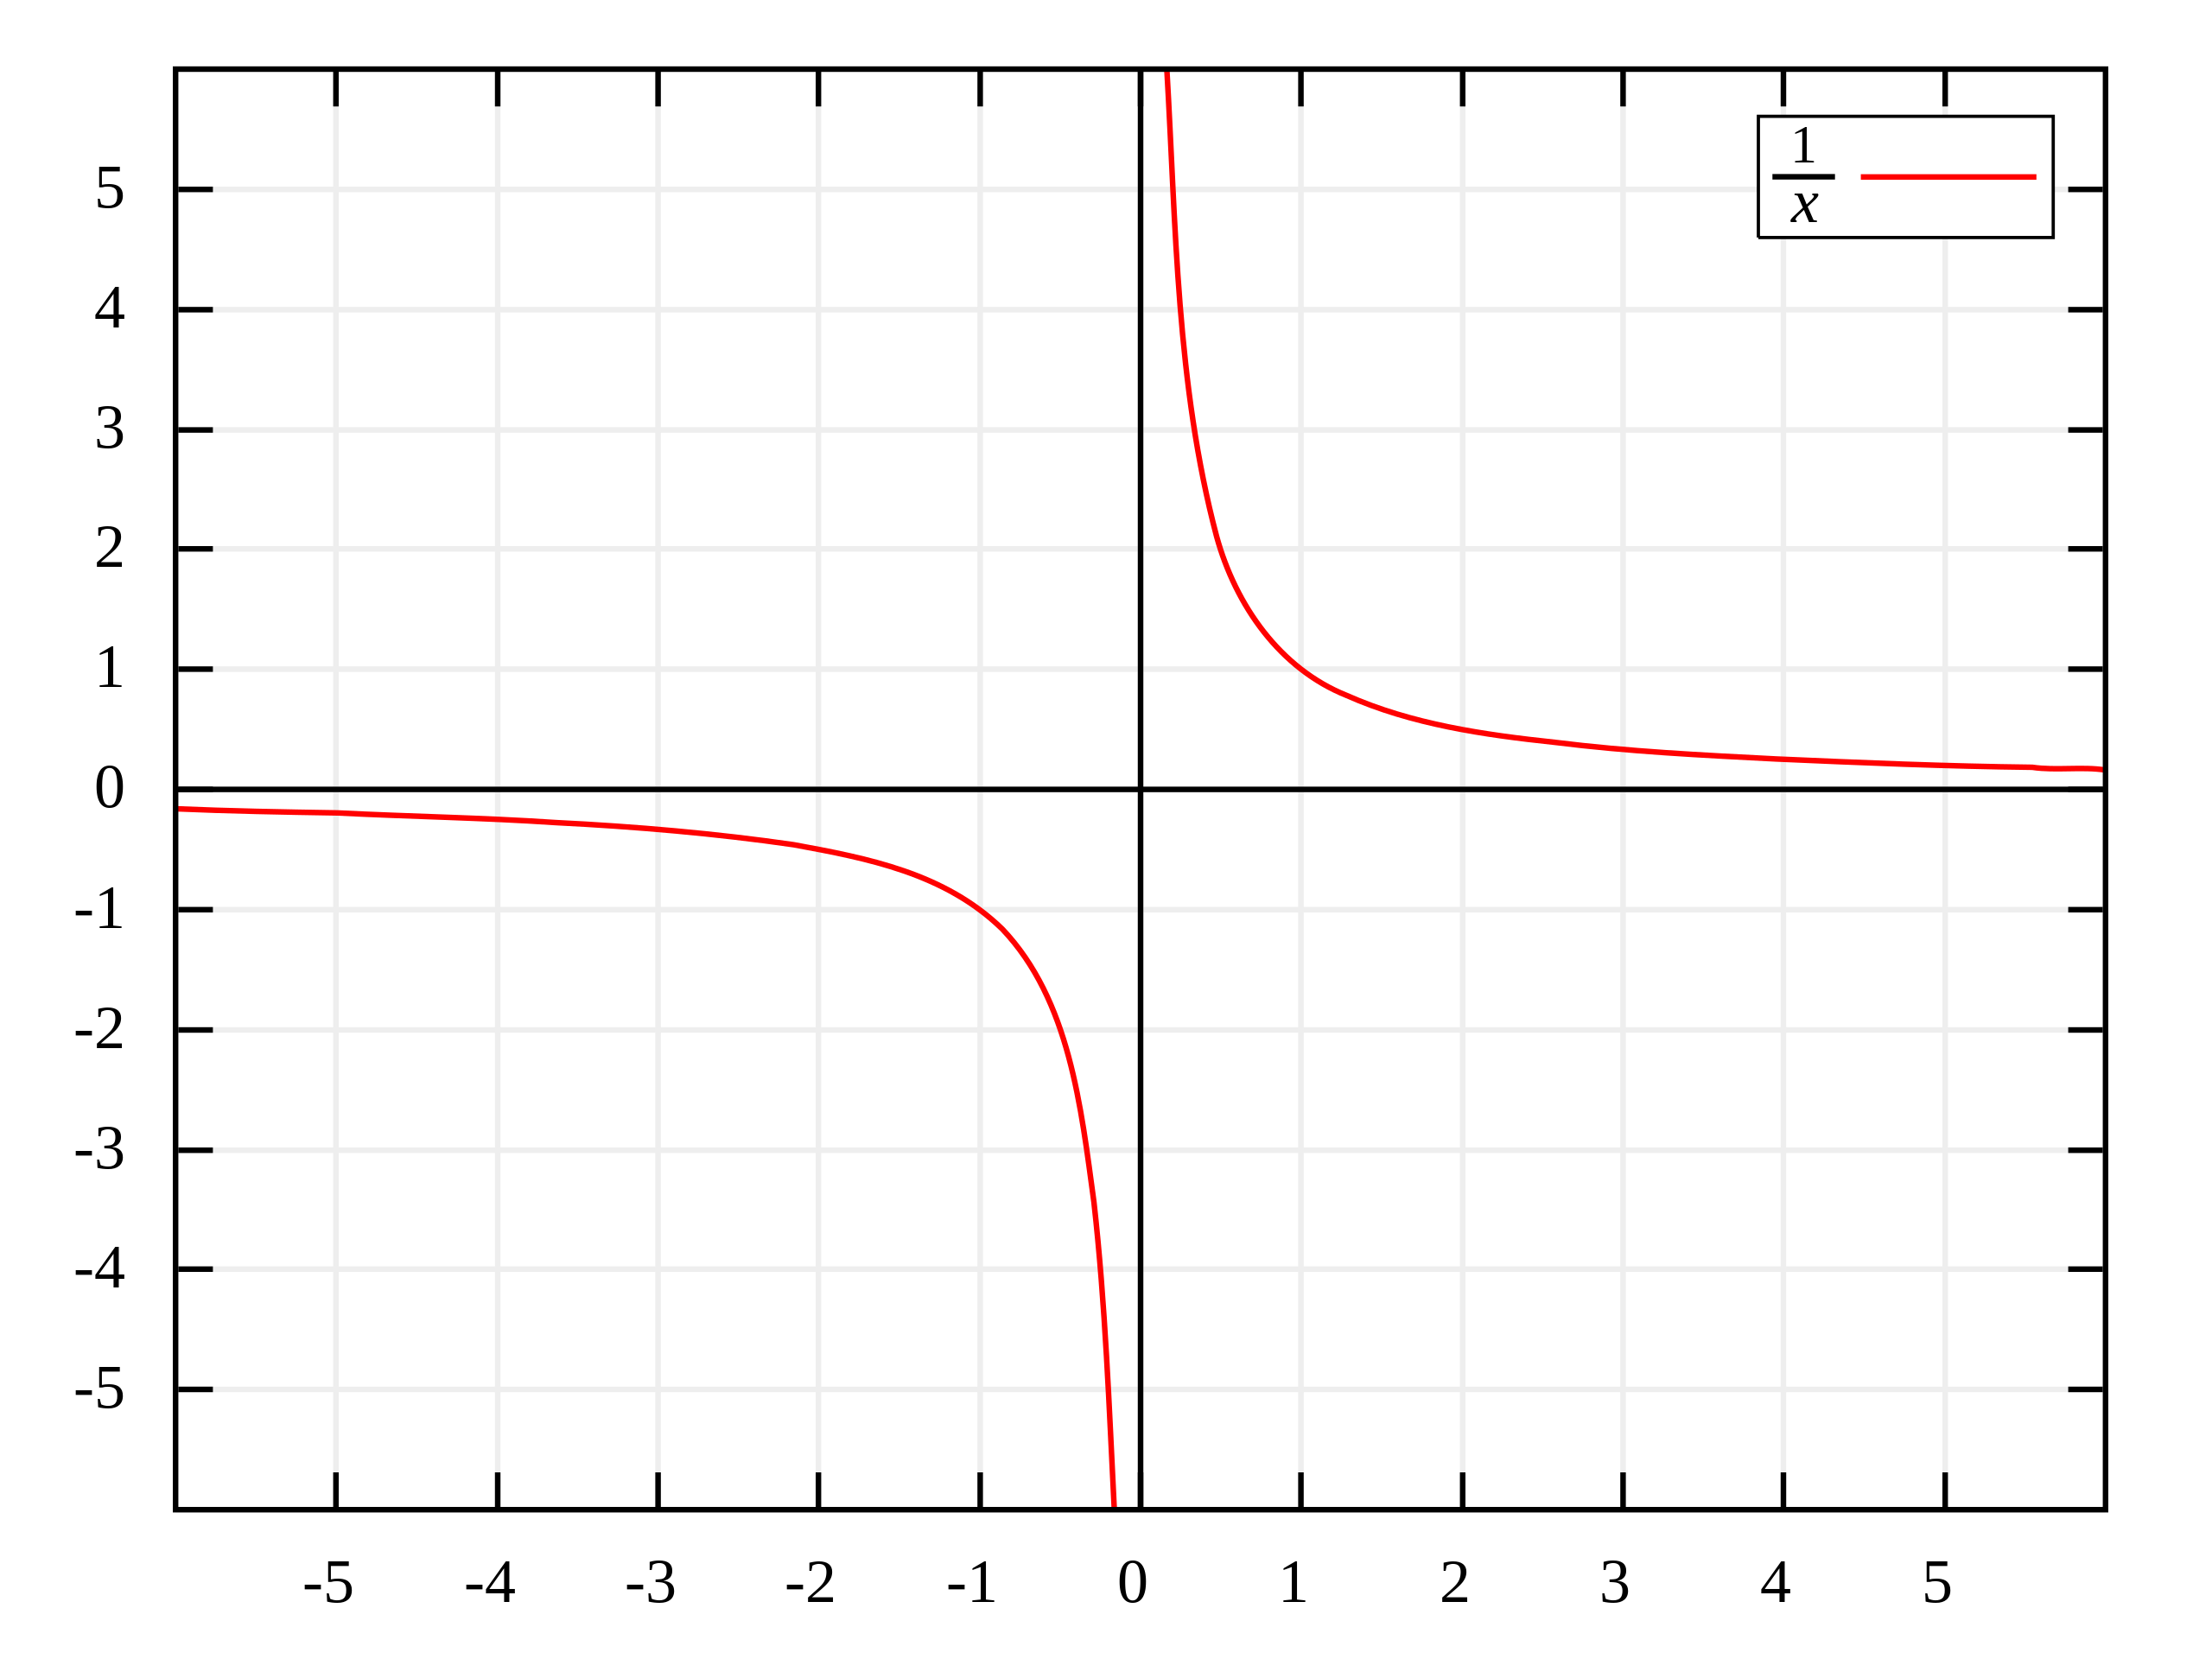
\includegraphics[trim={0 0 0 0.5cm},clip,scale=0.20]{sections/acm-template-sections/images/Hyperbola_one_over_x.svg.png}
    
    \caption{Explanation of division-by-zero error from wiki. (\url{https://upload.wikimedia.org/wikipedia/commons/4/43/Hyperbola_one_over_x.svg})}
    \label{fig:div-zero}
\end{figure*}
